\documentclass[12pt]{article}
\usepackage{amssymb}
\usepackage{amsmath}
\usepackage{amsthm}
\usepackage{mathtools}
\usepackage{array}
\usepackage{multirow}
\usepackage{colortbl}
\usepackage[dvipsnames]{xcolor}
\usepackage{graphicx}
  \DeclareGraphicsRule{*}{mps}{*}{}
%\usepackage{bbm}
\usepackage{marvosym}
\usepackage{enumerate}
\usepackage{txfonts}
\usepackage{paralist}
\usepackage{pdfpages}
\usepackage{multicol}
\usepackage{tikz}
\usepackage{siunitx}
\everymath{\displaystyle}

\usepackage[margin=.7in]{geometry}
%\usepackage{fullpage}

\setdefaultleftmargin{0pt}{}{}{}{}{}

\newcommand{\mblank}{\rule[-1ex]{8ex}{0.4pt}}
\definecolor{lightgray}{gray}{0.7}

\newenvironment{solution}
{\color{BrickRed}\textbf{Solution.} 
}
{\ignorespacesafterend}

% Circles for Venn diagrams
\def\firstcircle{(90:1cm) circle (1.5cm)}
\def\secondcircle{(210:1cm) circle (1.5cm)}
\def\thirdcircle{(330:1cm) circle (1.5cm)}


\renewcommand{\thefootnote}{\fnsymbol{footnote}}

\hyphenpenalty=5000
\tolerance=1000
\setlength{\parindent}{0pt}

\begin{document}
\pagestyle{empty}
\begin{center}
\section*{MATH 210 -- Chapter 3 quiz -- In-class portion}
\end{center}
\begin{enumerate}
	
\item %%%%%%%%%%%%%%% Translate, negate, translate back
\textbf{(L1, L3)}
This question will test your ability to go back and forth between the land of meaning and the land of symbols. Consider the following statement:
\begin{center}
	``Every number is either a multiple of 3, one more than a multiple of 3, or two more than a multiple of 3.''
\end{center}
\begin{enumerate}[(a)]
	\item Translate this statement into logical symbols.
	
	\item Write the \textbf{negation} of this statement in logical symbols. Simplify as much as possible.
	
	\item Translate your negation back into words.
	
\end{enumerate}

\item %%%%%%%%%%%%%%%%%%%%%%% Onto, one-one, translating
\textbf{(L1, S3)} Suppose that $f$ is a function with domain $A$ and codomain $B$.

\begin{enumerate}[(a)]
	\item
	Write the formal definition of $f$ being an \textbf{onto} function (also called a \textbf{surjective} function) using needed quantifiers and connectives.
	
	\item
	Assume that the domain $A$ and codomain $B$ for function $f$ are both finite sets and that $f$ is an onto function. What is the necessary relationship between the cardinality of $A$ and the cardinality of $B$?  Explain.
\end{enumerate}

	
\item %%%%%%%%%%%%%%%%%%%%%%% Translate for sets
\textbf{(S1)}
Recall that $\mathbb{Z}$ is the integers. Let $2\mathbb{Z}$ be the multiples of 2 and $3\mathbb{Z}$ be the multiples of 3, and so on.

\begin{enumerate}
	\item[a.]
	Find $\mathbb{Z} \setminus 2\mathbb{Z}$. Describe the set in words and using set-builder notation.
	
	\item[b.]
	Find $3\mathbb{Z} \cap 5\mathbb{Z}$. Describe the set in words and using set-builder notation. 
	
\end{enumerate}

\item %%%%%%%%%%%%%%%%%%%%%%% Venn diagrams
\textbf{(S2)} Consider the following Venn diagram:

\begin{center}
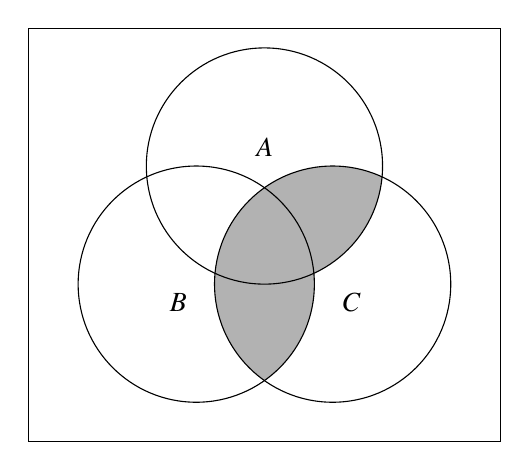
\begin{tikzpicture}
\begin{scope}
\clip \secondcircle;
\fill[lightgray] \thirdcircle;
\end{scope}
\begin{scope}
\clip \firstcircle;
\fill[lightgray] \thirdcircle;
\end{scope}
\draw \firstcircle node[text=black,above] {$A$};
\draw \secondcircle node [text=black,below left] {$B$};
\draw \thirdcircle node [text=black,below right] {$C$};
\draw (-3, -2.5) rectangle (3, 2.75);
\end{tikzpicture}
\end{center}

Describe the shaded area in \textbf{two different ways} using $A$, $B$, $C$, and set operations.


\item \textbf{(S4)} %%%%%%%%%%%%%%%%% Relations
Consider different possible relations $R$ on set $A=\{1,2,3,4,5\}$. Describe a relation $R$ on set $A$ with the following combinations of properties by stating $R$ as a set of ordered pairs and by illustrating $R$ with a directed graph.

\begin{enumerate}[(a)]
	\item
	$R$ is reflexive, is symmetric, and is not transitive
	
	\item
	$R$ is not reflexive, is symmetric, and is transitive
	
\end{enumerate}


\item %%%%%%%%%%%%%%%%%%%%%%%% Equivalence relations
\textbf{(S5)} Consider the relation on set $A=\{1,2,3,4\}$  illustrated below. 

\begin{figure}[!h]
	\centering
	\includegraphics[width=0.3\linewidth]{initial_relation.png}
	\caption{An initial relation on set $A$}
\end{figure}

\begin{enumerate}[(a)]
	\item
	Recall that an \textbf{equivalence relation} is one that is reflexive, symmetric, \textbf{and} transitive. Add the minimal number of directed edges to the relation to make it an equivalence relation.
	
	\item
	Given an equivalence relation $R$ on a set $A$, the equivalence class of an element $x$ in $A$ is written as $[x]$, and is defined as all the elements $y$ in $A$ such that $xRy$. For the equivalence relation you created in part (a), find all of the equivalence classes, that is, $[1]$, $[2]$, $[3]$, and $[4]$. 
	
\end{enumerate}

\section*{Take-home portion}
Finish up whichever of the above problems you didn't complete in class, and complete the problems below.

\item %%%%%%%%%%%%%%%%%%%%%%% Truth tables
\textbf{(L2)} Use a truth table to determine whether the following deduction rule is valid:
\[
\begin{array}{cc}
& P\to(Q\lor R) \\ 
& \lnot(P\to R) \\ \hline
\therefore & Q
\end{array} 
\]


\item %%%%%%%%%%%%%%%%%%%%%%% A proof
\textbf{(P1)}
If you multiply an odd number by an odd number, is the result even or odd? Prove your answer.


\item %%%%%%%%%%%%%%%%%%%%%% Disprove
\begin{enumerate}[(a)]
	\item \textbf{(P2)} To show that a universal statement (that is, one involving a $\forall$) is false, it's enough to give one counterexample, but to show that a universal statement is true, it's \textbf{not} enough to give one example. In your own words, explain why this is true.
	
	\item Prove or disprove: For all natural numbers $n$, if $n^2+n$ is even then $n$ is even.
	
\end{enumerate}


\end{enumerate}
\end{document}
